\documentclass[9pt]{beamer}
\usepackage{styles/mypreamble}
%~~~~~~~~~~~~~~~~~~~~~~~~~~~~~~~~~~~~~~~~~~~~~~~~~~~~~~~~~~~~~~~~~~~~~~~~~~~~~~
\title{Алгоритмы машинного обучения}
\subtitle{Лекция 3. Кластеризация}
\author{Владимир Кукушкин}
\institute{СПбГЭУ - 25.11.2020}
%~~~~~~~~~~~~~~~~~~~~~~~~~~~~~~~~~~~~~~~~~~~~~~~~~~~~~~~~~~~~~~~~~~~~~~~~~~~~~~

\begin{document}

\titlepage

\section{Постановка задачи кластеризации}

\begin{frame}
 \frametitle{Постановка задачи}
 \begin{itemize}
      \item Пусть есть датасет:
$$X = \begin{pmatrix}
x_{11} & \ldots & x_{1p} \\
\ldots & \ldots & \ldots \\
x_{N1} & \ldots & x_{Np}
\end{pmatrix}
$$
    \item \textbf{Задача:} Сгруппировать объекты $x_i$ по \textit{похожим} признакам.
    \item Более формально: построить отображение $C(x_i) = k$, где $k=1, \ldots, K$. $K$ -- некоторое (заранее не известное) число кластеров.
    \item Кластеризация -- это обучение без учителя
\end{itemize}
\end{frame}

\begin{frame}{Зачем нужна кластеризация}
\begin{itemize}
    \item Выявление паттернов в данных с целью выработки индивидуального подхода к каждой группе. В частности:
    \begin{itemize}
        \item Сегментация покупателей по отличительным признакам и моделям поведения.
        \item Сегментация данных для сжатия; храним информацию не о каждом объекте, а о группе).
        \item Сегментация данных для построения отдельных моделей классификации/регрессии.
    \end{itemize}
    \item Выделение нетипичных объектов.
    \item Построение иерархии множества объектов (задача таксономии).
\end{itemize}
\end{frame}

\begin{frame}{Особенности задачи классификации}
\begin{itemize}
    \item Не всё так однозначно (всё неоднозначно):
    \begin{itemize}
        \item Нет точной постановки задачи.
        \item Существует много (неоднозначных) критериев качества кластеризации.
        \item Существует много (неоднозначных) метрик в пространстве фичей, принципиально влияющих на результат кластеризации. 
        \item Количество кластеров, как правило, заранее неизвестно.
    \end{itemize}
    \item В итоге, разные методы могут приводить к разным результатам.
\end{itemize}
\end{frame}

\begin{frame}{Какие объекты похожи?}
\begin{itemize}
    \item Введём функцию $d_j$ расстояния между $j$-ми координатами двух точек $x_i, x_{i'}$. Она можеть быть разной для каждой фичи (или каждого типа фичи):
    \begin{itemize}
        \item Для непрерывных фичей:
        \begin{itemize}
            \item $d_j(x_{ij}, x_{i'j}) = (x_{ij} - x_{i'j})^2$,
            \item $d_j(x_{ij}, x_{i'j}) = l(|x_{ij} - x_{i'j}|)$, где $l$ -- дополнительная функция штрафа за удалённость.
        \end{itemize}
        \item Для порядковых фичей:
        \begin{itemize}
            \item Заменяем значение $x_{ij}$ на $\frac{x_{ij} - 1/2}{M}$, где $M$ -- количество возможных значений фичи.
            А дальше обращаемся, как с непрерывной.
        \end{itemize}
        \item Для категориальных фичей:
        \begin{itemize}
            \item $d_j(x_{ij}, x_{i'j}) = \mathds{1}(x_{ij} \neq x_{i'j})$,
            \item Или явно определяем матрицу расстояний между всеми возможными значениями фичи.
        \end{itemize}
    \end{itemize}
\end{itemize}
\end{frame}

\begin{frame}{Какие объекты похожи?}
\begin{itemize}
    \item Теперь можно задать расстояние между двумя точками как $$D(x_i, x_{i'}) = \sum\limits_{j=1}^p d_j(x_{ij}, x_{i'j})$$
    \item Или в более общем случае:
    $$D(x_i, x_{i'}) = \sum\limits_{j=1}^p w_j \cdot d_j(x_{ij}, x_{i'j}), \;\;\; \sum\limits_{j=1}^p w_j=1$$
    \item Веса $w_j$ можно задавать пропорционально дисперсии фичи (почему?)
\end{itemize}
\end{frame}

\begin{frame}{Практические советы}
\begin{itemize}
    \item Выбор функции $D(x_i, x_{i'})$ критично влияет на качество кластеризации.
    \item Как заменять пропущенные значения (NA)?
    \begin{itemize}
        \item Выкинуть все точки, где есть хотя бы одно NA
        \item Заменить на средние
        \item Для категориальных ввести специальную категорию NA
    \end{itemize}
    \item Вместо выбора весов $w_j$ можно использовать стандартизацию данных:
    $$\tilde x_{ij} = \frac{x_{ij} - \bar X_j}{\sigma_j}$$
\end{itemize}
\end{frame}

\begin{frame}{Пример о пользе стандартизации}
\begin{itemize}
    \item<1-> Пусть в первом датасете фича $X_1$ исчисляется в сантиметрах, во второй -- в метрах.
    \begin{center}
    \begin{tabular}{c|c|c}
        & $X_1$ & $X_2$ \\
        \hline
        $x_1$ & 10 & 1 \\
        $x_2$ & 20 & 3 \\
        $x_3$ & 30 & 2 \\
    \end{tabular}\quad\quad\quad\quad\quad\quad\quad\quad
    \begin{tabular}{c|c|c}
        & $X_1$ & $X_2$ \\
        \hline
        $x'_1$ & 0.1 & 1 \\
        $x'_2$ & 0.2 & 3 \\
        $x'_3$ & 0.3 & 2 \\
    \end{tabular}
    \end{center}

    \pause

    \resizebox{\textwidth}{!}{%
    \begin{tabular}{cc}
    $\begin{array}{rl}d(x_1, x_2) &= (20-10)^2 + (3-1)^2 =\\&= 104 \end{array}$ &
    $\begin{array}{rl}d(x'_1, x'_2) &= (0.2-0.1)^2 + (3-1)^2 =\\&= 4.01 \end{array}$\\
    $\begin{array}{rl}d(x_1, x_3) &= (30-10)^2 + (2-1)^2 =\\&= 401 \end{array}$ &
    $\begin{array}{rl}d(x'_1, x'_3) &= (0.3-0.1)^2 + (2-1)^2 =\\&= 1.04 \end{array}$ \vspace{0.3cm}\\
    $d(x_1, x_2) < d(x_1, x_3)$ & $d(x'_1, x'_2) > d(x'_1, x'_3)$
    \end{tabular}%
    }
    \item Стандартизация избавит непрерывные фичи от таких недостатков. Но с дискретными всё равно будут сложности.
\end{itemize}
\end{frame}

\begin{frame}{Качество кластеризации}
$$W(C) = \frac{1}{2}\sum_{k=1}^K\sum_{C(i)=k}\sum_{C(i')=k}d(x_i, x_{i'}) \text{ -- внутрикластерные расстояния},$$
$$B(C) = \frac{1}{2}\sum_{k=1}^K\sum_{C(i)=k}\sum_{C(i')\neq k}d(x_i, x_{i'}) \text{ -- внешнекластерные расстояния}$$.

\begin{itemize}
    \item Чем кластер плотнее, тем меньше $W(C)$.
    \item Чем кластеры дальше разделены друг от друга, тем больше $B(C)$.
    \item Значит, можно либо минимизировать $W(C)$, либо максимизировать $B(C)$.
    \item Но это эквивалентные задачи, и вот почему:
\end{itemize}
$$T = \frac{1}{2}\sum_{i=1}^N\sum_{i'=1}^N d_{ii'} = \frac{1}{2}\sum_{k=1}^K\sum_{C(i)=k}\left(\sum_{C(i')=k} d_{ii'} + \sum_{C(i')\neq k} d_{ii'} \right) = W(C) + B(C)$$
\;\;\;\;\;($T$ -- константа, и не зависит от кластеризации).
    
\end{frame}

\begin{frame}{Почему не брутфорс?}
\begin{itemize}
    \item Идея: переберём все варианты кластеризации, найдём минимум $W(C)$.
    \item Сколько различных вариантов распределить $N$ точек по $K$ кластерам?
    $$S(N, K) = \frac{1}{K!}\sum_{k=1}^K(-1)^{K-k}C_K^k k^N$$
    \item $S(10, 4) = 34105$, $S(19, 4)=10^{10}.$
\end{itemize}
\end{frame}

\section{Алгоритм K-means}

\begin{frame}{Начальная конфигурация}
\begin{itemize}
    \item Предполагаем, что находимся в евклидовом пространстве (то есть $d(x_i, x_{i'}) = \sum\limits_{j=1}^p (x_{ij} - x_{i'j})^2 = \|x_i-x_{i'}\|^2$).
    \item Тогда внутрикластерное расстояние будет выглядеть так (\href{https://en.wikipedia.org/wiki/Variance\#Population_variance}{См. похожее объяснение}):
    $$W(C) = \frac{1}{2}\sum_{k=1}^K\sum_{C(i)=k}\sum_{C(i')=k}\|x_i - x_{i'}\|^2 = \sum_{k=1}^K N_k\sum_{C(i)=k} \|x_i-\bar x_k\|^2\xrightarrow{C} \min.$$
    \item $\forall S \;\;\bar x_S = \underset{m}{\operatorname{argmin}}\sum\limits_{i\in S}\|x_i-m\|^2.$
\end{itemize}
    
\end{frame}

\begin{frame}{Идея алгоритма}
    \begin{enumerate}
        \item Задаём количество кластеров.
        \item Инициализация. Выбираем центры кластеров случайно.
        \item Кластеризация. Относим точки тому кластеру, к центру которого они находятся ближе всего.
        \item Пересчитываем центры у получившихся кластеров.
        \item Повторяем п.3, 4 до сходимости.
    \end{enumerate}
\end{frame}

\framedgraphic{Иллюстрация}{img/kmeans.png}

\begin{frame}{Плюсы, минусы, подводные камни}
\begin{itemize}
    \item  Один из самых популярных методов.
    \item Находит только локальный экстремум.
    \item Ориентируется на шарообразные кластеры. Не позволяет выявлять ленточные кластеры.
    \item Сложность $O(KNp)$.
    \item Зависит от начального положения центров.
\end{itemize}
\end{frame}

\framedgraphic{Проблема с инициализацией центров}{img/kmeans_initialization_trap.png}

\begin{frame}{Как тогда инициализировать центры?}
\begin{itemize}
    \item Рандомно. Назначаем точки в кластеры рандомно, находим их центры.
    \item Метод Forgy. Центры -- случайные $K$ точек датасета.
\end{itemize}
\end{frame}

\begin{frame}{Инициализация центров. Метод kmeans++.}
\begin{itemize}
    \item kmeans++ -- улучшенный метод Forgy.
\end{itemize}
\begin{enumerate}
    \item Первый центр выбираем случайно.
    \item Для каждой точки считаем $d^2$ до ближайшего центра.
    \item Выбираем новый центр среди точек случайно с вероятностями, пропорциональными $d^2$.
    \item Повторяем п.2,3, пока не наберём $K$ центров.
\end{enumerate}
\begin{itemize}
    \item После такого назначения центров, запускаем основной K-means.
    \item В среднем kmeans++ позволяет работать всей кластеризации быстрее.
\end{itemize}
\end{frame}

\begin{frame}{Как определить $K$?}
    \begin{itemize}
        \item Здесь уже поможет брутфорс.
        \item Пробуем несколько $K$, строим график $W(K)$ (a.k.a каменистая осыпь, правило локтя).
        \item Там, где выходим на горизонталь, там оптимальное количество кластеров.
    \end{itemize}
\begin{center}
    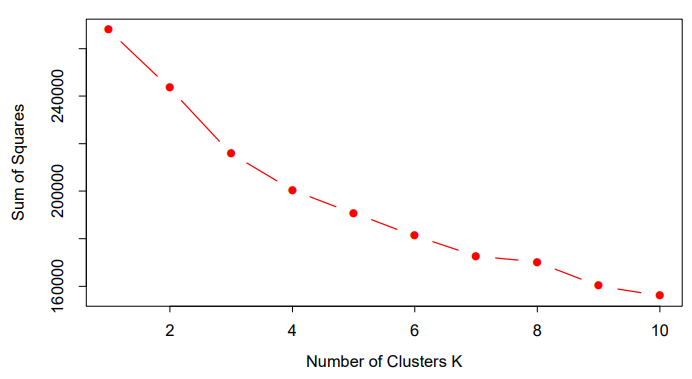
\includegraphics[height=5cm]{img/elbow_rule.png}
\end{center}
\end{frame}

\begin{frame}{Ещё пара проблем}
\textbf{Q:} Алгоритм находит локальный минимум. Что делать?\\
\textbf{A:} Стандартный способ: запускать его несколько раз с разных начальных точек.

\textbf{Q:} Как понять, что кластеризация получилась действительно хорошая?\\
\textbf{A:} Только вручную интерпретируя результаты.
\end{frame}

\section{Иерархическая кластеризация}

\begin{frame}{Предпосылки и идея алгоритма}
\begin{itemize}
    \item В K-means нам не нравилось, что результат зависел от инициализации центров.
    \item Что если отказаться от изначального задания центров вообще?
    \item Будем на строить иерархию объектов: на нижнем уровне индивидуальные точки, на верхнем -- один большой кластер из всех точек. Всего $N-1$ уровней.
    \item Иерархию можно строить:
    \begin{itemize}
        \item Либо вверх, объединяя мелкие кластеры в более крупные, начиная с индивидуальных точек.
        \item Либо вниз, разделяя крупные кластеры на более мелкие, начиная со всего датасета.
    \end{itemize}
    \item На каждом шаге будем принимать решение, какие два кластера наиболее достойны объединения/разбиения.
    \item Обычно иерархию строят вверх, а не вниз.
\end{itemize}
\end{frame}

\begin{frame}{Дендрограмма}
    \begin{itemize}
        \item Дендрограмма -- естественный способ визуализации иерархии данных.
        \item Длина каждого вертикального ребра пропорциональна близости объединяемых кластеров.
        \item Можно визуально определить, сколько кластеров должно быть в итоге.
    \end{itemize}
    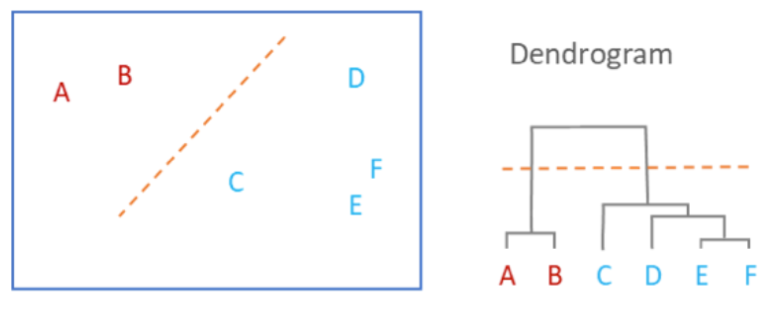
\includegraphics[width=\textwidth]{img/dendrogram_example.png}
\end{frame}

\begin{frame}{Что такое близость кластеров?}
Пусть есть два кластера $G$ и $H$. Расстояние между ними можно определить по-разному.
$$d_{SL} = \min_{i\in G, i'\in H} d(x_i, x_{i'}) \text{ -- Single Linkage, a.k.a. nearest-neighbor},$$
$$d_{CL} = \max_{i\in G, i'\in H} d(x_i, x_{i'}) \text{ -- Complete Linkage, a.k.a. furthest-neighbor},$$
$$d_{GA} = \frac{1}{|G||H|}\sum_{i\in G}\sum_{x_i'\in H}d(i, x_{i'})\text{ -- Group Average},$$
$$d_{W} = \sum_{i\in G\cup H}\|x_i - m_{G \cup H}\|^2 - \sum_{i\in G}\|x_i - m_G\|^2 - \sum_{i\in H}\|x_i - m_H\|^2\text{ -- Ward}.$$
\end{frame}

\begin{frame}{Особенности межкластерных расстояний}
$$D_G = \max_{i\in, i'\in G} d(i, i') \text{ -- диаметр кластера G}.$$
    \begin{itemize}
        \item Single linkage: достаточно только пары близких точек, чтобы кластеры считались близкими. Приводит к т.н. chaining problem: кластеры становятся вытянутыми и расползаются. Диаметр получающихся кластеров будет  большим.
        \item Complete linkage: кластеры будут близкими только если все точки будут близкими. Диаметр получающихся кластеров будет маленьким (может это и не плохо).
        \item Group average: компромиссное решение.
    \end{itemize}
Зато Single linkage и Complete linkage не зависят от размерности данных, а group average чувствителен к этому. Но мы же не будем никогда запускать кластеризацию без стандартизации?
\end{frame}

\framedgraphic{Как влияет выбор метрики}{img/dendrogram_dissimilarities.png}

\begin{frame}{Плюсы, минусы, подводные камни}
    \begin{itemize}
        \item Позволяет отобразить структуру данных.
        \item Сложность $O(N^3)$, да ещё и $O(N^2)$ памяти. Иногда сложность можно понизить до $O(N^2)$. 
    \end{itemize}
\end{frame}

\begin{frame}[allowframebreaks]
    \frametitle{Литература}
    \bibliographystyle{unsrt}
    \nocite{esl, kmeanspp}
    \bibliography{references.bib}
\end{frame}

\end{document}